%!TEX root = ../masters_thesis.tex

\chapter{Concept} % (fold)
\label{cha:concept}

The first section of this chapter explains the spatio-temporal data model developed in this thesis and the related concepts of an  \emph{Hivent} and an \emph{Area}. It shows ten \emph{Historical Geographic Operations} that represent all kinds of changes that can happen in the development of a country. The second section introduces \emph{HistoGlobe}, the application used in this thesis. The chapter finishes with the \emph{EditMode} and the \emph{HistoGraph} as interface extensions to HistoGlobe to visualize and edit historical changes of countries.

% - - - - - - - - - - - - - - - - - - - - - - - - - - - - - - - - - - - - - - -
\paragraph{Area identity} % (fold)
\label{par:area_identity}

Given the example of Germany, the Area is independent from both its territory and short name: In 1949, four years after the end of World War II, the German Democratic Republic (\emph{East Germany}) and the Federal Republic of Germany (\emph{West Germany}) were created. In 1957, the Saar Protectorate (\emph{Saarland}) joined West Germany. Although the territory of the Area has changed, it is still the same Area. In 1990, East and West Germany reunited to what is currently known as Germany. This Germany is still the Federal Republic of Germany, so it is juristically the same as West Germany before 1990. That means that also the short name of an Area can change (West Germany to Germany) without affecting the identity of the Area.


% paragraph area_identity (end)

% - - - - - - - - - - - - - - - - - - - - - - - - - - - - - - - - - - - - - - -
\paragraph{Historical Geographic Operations} % (fold)
\label{par:historical_geographic_operations}


\begin{enumerate}

  \item Identity-changing operations for one Area
  \begin{description}
    \item[CRE -- Creation]
    A new Area is created with a new name and a new territory fully on previously unclaimed land. \\
    \begin{footnotesize}
      The Roman Kingdom (753 - 509 B.C.) was created in Latinum, today central Italy, in a region that did not have anything before which would be considered a political entity.
    \end{footnotesize}
    \item[ICH -- Identity Change]
    The formal name of an Area changes, therefore the old Area is destructed and a new Area with the same territory is created. The old Area is the historical predecessor of the new Area. \\
    \begin{footnotesize}
      In the end of the Cold War, the Polish People's Republic (1952-1989) got renamed to present-day Republic of Poland (since 1989). Although the short name (Poland) stayed, the new country is a new political entity and is therefore to be modeled a new Area.
    \end{footnotesize}
    \item[CES -- Cessation]
    An Area stops to exist and ceases, leaving unclaimed land. Cessation is the inverse operation of Creation. \\
    \begin{footnotesize}
      The Minoan civilisation, populating the nowadays Greek island of Crete (3650 to 1400 B.C.) declined and left no immediate successor.
    \end{footnotesize}
  \end{description}

  \item Identity-changing operations for two or more Area
  \begin{description}
    \item[UNI -- Unification]
    Two or more old Areas unify to a new Area. The old Areas cease, becoming the historical predecessors of the new Area. It receives a new name and its is the union of the territories of the old Areas. \\
    \begin{footnotesize}
      In 1922, the Russian SFSR, the Transcaucasian SFSR, the Ukrainian SSR and the Byelorussian SSR unified and formed the Union of Soviet Socialist Republics (USSR).
    \end{footnotesize}
    \item[INC -- Incorporation]
    One or more old Areas are incorporated into another Area. This areas preserves its identity, i.e. formal name, but may get a new short name. Its territory in enlarged by the union of the old Areas. The old Areas are historical predecessors of the new Area. \\
    \begin{footnotesize}
      In 1990, the territory of the German Democratic Republic (East Germany) became part of the Federal Republic of Germany (West Germany). Although this event is known as the \emph{German Reunification}, it is historically an incorporation of East Germany into West Germany \cite{incorporationEastWestGermany}. Additionally, the commonly known short name of West Germany got changed into Germany, creating the country existing until today.
    \end{footnotesize}
    \item[SEP -- Separation]
    As the inverse of unification, one old Area is preceded by two or more new Areas. Each new Area gets a new name, receives a part of the territory of the old Area, and the old Area as the historical predecessor. \\
    \begin{footnotesize}
      In 1993, the Czech and Slovak Federal Republic, commonly known as Czechoslovakia, dissolved into present-day Czech Republic and Solvak Republic, creating two new countries.
    \end{footnotesize}
    \item[SEC -- Secession]
    As the inverse of incorporation, one or more new areas are ceded from a previously exising area. This Area may receive a new short name, but keeps its formal name and therefore its identity. Each new Area gets a new name, receives the previously existing Area as the historical predecessor and a part of its territory. \\
    \begin{footnotesize}
      In 2008, the Republic of Kosovo declared independence from Serbia and has since then partially received international recognition, so it can be seen as a new country. Unlike in the case of separation, Serbia kept its name, but ceded only a part of its territory to Kosovo. Therefore, Serbia kept its identity and keeps on existing.
    \end{footnotesize}
  \end{description}

  \item Identity-preserving operations for one or more Areas
  \begin{description}
    \item[BCH -- Border Change]
    Parts of the territory of one Area is ceded to one of its neighors. Therefore, the border shared by two neighboring Areas changes. The names of the two Areas remain unchanged. Geographically, this operation preserves also the topology: Since only the border between two countries changes, they are still neighboring like before. \\
    \begin{footnotesize}
      As the result of the Treaty of Versailles in 1919, the German Empire ceded 13 \% of its territory, e.g. Alsace-Lorraine to France, changing the German-French border.
    \end{footnotesize}
    \item[TCH -- Territory Change]
    A territory change is a special case of a border change: The territory of an Area is partially expanding into previously unclaimed land or partially shrinking, leaving unclaimed land. \\
    \begin{footnotesize}
      Throughout the British Colonization of North America, several settlements and later colonies, e.g. in 1607 the colony of Virginia, were found. Their territory was often expanded westwards, incorporating previously unclaimed land.
    \end{footnotesize}
    \item[NCH -- Name Change]
    An Area changes its short name. Its territory, formal name and identity is preserved. \\
    \begin{footnotesize}
      The most recent geopolitical change happened on 5. May 2016, when the cabinet of Czech Republic approved that the country will now offically be called ``Czechia''. However, the formal name stays Czech Republic.
    \end{footnotesize}
  \end{description}
\end{enumerate}

\begin{table}[!h]
\begin{center}
\begin{tabular}{m{0.65cm} m{2.5cm} m{2.2cm}
                m{0.35cm} m{0.35cm} m{0.35cm} m{0.01cm}
                m{0.35cm} m{0.3cm} m{0.35cm} m{0.01cm}
                m{0.35cm} m{0.3cm} m{0.88cm}}
  \toprule
    \multicolumn{2}{c}{operation}
  & visualization
  & \multicolumn{e3}{c}{Area change} &
  & \multicolumn{3}{c}{name change} &
  & \multicolumn{3}{c}{territory change} \\
  & & &
  old & $ \leftrightarrow_H $ & new & &
  old & $ \rightarrow $ & new & &
  old & $ \rightarrow $ & new \\

  \midrule[0.07em]
  \texttt{CRE} & Creation & 
\includegraphics{graphics/concept/operations/CRE} &
  $ \emptyset $ & $ \rightarrow $ & $ A $ & &
  $ \emptyset $ & $ \rightarrow $ & $ A_N $ & &
  $ \emptyset $ & $ \rightarrow $ & $ A_T $ \\

  \midrule[0.01em]
  \texttt{ICH} & Identity Change & 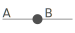
\includegraphics{graphics/concept/operations/ICH} &
  $ A   $ & $ \leftrightarrow_H $ & $ B $ & &
  $ A_N $ & $ \rightarrow $       & $ B_N $ & &
  $ A_T $ & $ \rightarrow $       & $ B_T $ \\

  \midrule[0.01em]
  \texttt{CES} & Cessation & 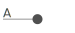
\includegraphics{graphics/concept/operations/CES} &
  $ A $   & $ \rightarrow $       & $ \emptyset $ & &
  $ A_N $ & $ \rightarrow $       & $ \emptyset $ & &
  $ A_T $ & $ \rightarrow $       & $ \emptyset $ \\

  \midrule[0.07em]
  \multirow{3}{*}{\texttt{UNI}} &
  \multirow{3}{*}{Unification} &
  \multirow{3}{*}{
\includegraphics{graphics/concept/operations/UNI}} &
  $ A $   & $ \leftrightarrow_H $ & $ C $ & &
  $ A_N $ & $ \rightarrow $       & $ \emptyset $ & &
  $ A_T $ & $ \rightarrow $       & $ \emptyset $ \\
  & & &
  $ B $   & $ \leftrightarrow_H $ & $ C $ & &
  $ B_N $ & $ \rightarrow $       & $ \emptyset $ & &
  $ B_T $ & $ \rightarrow $       & $ \emptyset $ \\
  & & &
  & & & &
  $ \emptyset $ & $ \rightarrow $ & $ C_N $ & &
  $ \emptyset $ & $ \rightarrow $ & $ C_T $ \footnotemark \\

  \midrule[0.01em]
  \multirow{2}{*}{\texttt{INC}} &
  \multirow{2}{*}{Incorporation} &
  \multirow{2}{*}{\includegraphics{graphics/concept/operations/INC}} &
  & & & &
  $ (A_N $ & $ \rightarrow $      & $ A_{N'}) $ & &
  $ A_T $ & $ \rightarrow $       & $ A_{T'} $ \footnotemark \\
  & & &
  $ B $   & $ \leftrightarrow_H $ & $ A $ & &
  $ B_N $ & $ \rightarrow $       & $ \emptyset $ & &
  $ B_T $ & $ \rightarrow $       & $ \emptyset $ \\

  \midrule[0.01em]
  \multirow{3}{*}{\texttt{SEP}} &
  \multirow{3}{*}{Separation} &
  \multirow{3}{*}{
\includegraphics{graphics/concept/operations/SEP}} &
  $ A $         & $ \leftrightarrow_H $ & $ B $ & &
  $ A_N $       & $ \rightarrow $       & $ \emptyset $ & &
  $ A_T $       & $ \rightarrow $       & $ \emptyset $ \\
  & & &
  $ A $         & $ \leftrightarrow_H $ & $ C $ & &
  $ \emptyset $ & $ \rightarrow $       & $ B_N $ & &
  $ \emptyset $ & $ \rightarrow $       & $ B_T $ \\
  & & &
  & & & &
  $ \emptyset $ & $ \rightarrow $       & $ C_N $ & &
  $ \emptyset $ & $ \rightarrow $       & $ C_T $ \footnotemark \\

  \midrule[0.01em]
  \multirow{2}{*}{\texttt{SEC}} &
  \multirow{2}{*}{Secession} &
  \multirow{2}{*}{\includegraphics{graphics/concept/operations/SEC}} &
  $ A $     & $ \leftrightarrow_H $     & $ B $ & &
  $ (A_N $  & $ \rightarrow $           & $ A_{N'}) $ & &
  $ A_T $   & $ \rightarrow $           & $ A_{T'} $ \\
  & & &
  & & & &
  $ \emptyset $ & $ \rightarrow $ & $ B_N $ & &
  $ \emptyset $ & $ \rightarrow $ & $ B_T $ \footnotemark \\

  \midrule[0.07em]
  \multirow{1}{*}{\texttt{NCH}} &
  \multirow{1}{*}{Name Change} &
  \multirow{1}{*}{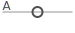
\includegraphics{graphics/concept/operations/NCH_TCH}} &
  & & & &
  $ A_N $ & $ \rightarrow $ & $ A_{N'} $ & &
  & & \\

  \midrule[0.01em]
  \multirow{2}{*}{\texttt{BCH}} &
  \multirow{2}{*}{Border Change} &
  \multirow{2}{*}{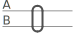
\includegraphics{graphics/concept/operations/BCH}} &
  & & & &
  & & & &
  $ A_T $ & $ \rightarrow $ & $ A_{T'} $ \\
  & & &
  & & & &
  & & & &
  $ B_T $ & $ \rightarrow $ & $ B_{T'} $ \footnotemark \\

  \midrule[0.01em]
  \multirow{1}{*}{\texttt{TCH}} &
  \multirow{1}{*}{Territory Change} &
  \multirow{1}{*}{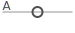
\includegraphics{graphics/concept/operations/NCH_TCH}} &
  & & & &
  & & & &
  $ A_T $ & $ \rightarrow $ & $ A_{T'} $ \\

  \bottomrule
\end{tabular}
\caption{Overview about all 10 historical geographic operations}
\small{$A \leftrightarrow_H B$ denotes historical relationship between two Areas, \\ i.e. $A$ is predecessor of $B$ and $B$ is successor of $A$}
\label{tab:historical_geographic_operations}
\end{center}
\end{table}

\addtocounter{footnote}{-4}
\footnotetext{$C_{T} = A_T \cup B_T$}
\addtocounter{footnote}{1}
\footnotetext{$A_{T'} = A_T \cup B_T$}
\addtocounter{footnote}{1}
\footnotetext{$B_T \cup C_{T} = A_T$}
\addtocounter{footnote}{1}
\footnotetext{$A_{T'} \cup B_{T} = A_T$}
\addtocounter{footnote}{1}
\footnotetext{$A_{T} \cup B_{T} = A_{T'} \cup B_{T'}$}

% paragraph historical_geographic_operations (end)

% - - - - - - - - - - - - - - - - - - - - - - - - - - - - - - - - - - - - - - -
\paragraph{MECE principle} % (fold)
\label{par:mece_principle}

The MECE principle -- mutually exclusive and collectively exhaustive -- is used by the consulting company McKinsey for organizing large amounts of data and as a strategy for effective problem solving. The advantages of a MECE model are \cite{mece}:
\begin{itemize}
  \item Each possible case in the real world can be mapped to a case in the model, because the model covers all possibilities (\emph{collectively exhaustive}).
  \item A case in the real world can be expressed by exactly one case in the model, because there is only one possibility (\emph{mutually exclusive}).
  \item The model is logical and comprehensive, can easily be understood and followed.
\end{itemize}

% paragraph mece_principle (end)

% - - - - - - - - - - - - - - - - - - - - - - - - - - - - - - - - - - - - - - -
\paragraph{Mutual exclusion} % (fold)
\label{par:mutual_exclusion}

First it is to be shown that one operation can not be equivalently expressed by a combination of any other operations. This is obviously true for \texttt{CRE}, because all other operations require at least one old area as an input to the operation. Vice versa, \texttt{CES} is unique, because it is the only operation without any new areas. \texttt{ICH} could geographically be represented by a combination of \texttt{CES} of and \texttt{CRE}, but that would not create a historical relationship between both Areas. Since the other identity-changing operations require either multiple old or new areas and the last three operations are identity-preserving, \texttt{ICH} is also unique.

\texttt{UNI}, \texttt{INC}, \texttt{SEP} and \texttt{SEC} require either old or new areas and establish historical relationships by changing identities. That is why they can neither be replaced by \texttt{CRE}, \texttt{ICH} and \texttt{CES} (only one old and/or new area), nor by \texttt{NCH}, \texttt{BCH} and \texttt{TCH} (identity-preserving). It is trivial that no operation can be expressed by its inverse and an operation that requires one old area can not replaced by one that requires multiple and vice versa. Therefore, the only possible combinations left are \texttt{UNI} $\leftrightarrow$ \texttt{INC} and \texttt{SEP} $\leftrightarrow$ \texttt{SEC}. While geographically, they are equivalent, because they unite respectively separate the territory in the same way, they are historically distinct: While in \texttt{UNI} and \texttt{SEP}, no Area is preserved in the operation, \texttt{INC} and \texttt{SEC} represent one Area that incorporate one Area into respectively cede one Area from its own territory. This shows the mutual exclulsion of all identity-preserving operations.

It has already been argued that identity-preserving operations can not be expressed by a combination of any identity-changing ones. Also, \texttt{NCH} changes the name, whereas \texttt{TCH} and \texttt{BCH} manipulate the territory of an Area, so it is clear they can not replace each other. By intuition, \texttt{BCH} is the same as two \texttt{TCH} of both Areas affected by the \texttt{BCH}. Both operations do also not set up any historical relationship, so they are historically the same. However, geographically, two \texttt{TCH} of two neighboring countries would be redundant, since the territory ceded by one Area is exactly the same territory that is incorporate by the neighbor. Therefore it has been proofed that all operations are mututally exclusive.

% paragraph mutual_exclusion (end)

% - - - - - - - - - - - - - - - - - - - - - - - - - - - - - - - - - - - - - - -
\paragraph{Exhaustive collection} % (fold)
\label{par:exhaustive_collection}

Next it needs to be shown that all cases that can happen in the real world can be expressed using a combination of one of the ten HG Operations. The first aspect is the identity of an Area, representing a political entity in the real world. In the life cycle of an entity, it is established at one point $t_s$, its name and territory can change multiple times while being active $U: \forall t_u \in U: t_u > t_s$ and it ceases at some other point $t_e: t_s < \forall t_u \in U < t_e$.



In the real world, a political entity can be created in three ways:
\begin{enumerate}
  \item If before the creation of the entity its initial territory was fully unclaimed, it does it have any historical predecessors and is created new. This is represented in the \texttt{CRE} operation.
  \item If its initial territory was fully claimed by a set of entities, then all of these entities are historical predecessors.
  \begin{enumerate}
    \item If the entity originates from itself by changing its formal name, the territory remains unchanged. The \texttt{ICH} operation reflects that case.
    \item An entitiy can also originiate from one entity that has dissolved into several subsequent entities, which is represented in the \texttt{SEP} operation.
    \item Finally, an entity can originate from several entities unifying. The \texttt{UNI} operation models this case.
  \end{enumerate}
  \item If the new entities territory was partially claimed and partially unclaimed, this process of creating entity $A$ can be expressed by a combination of three operations:
  \begin{enumerate}
    \item \texttt{CRE} creates the temporary entity $A_T$ with a new name and its territory on all unclaimed land that shall be occupied by $A$ later.
    \item The rest is currently territory of a set of entities $B$. For each entity $B_i \in B$, the part that shall be territory of $A$ gets ceded from $B_i$ with a \texttt{SEC} operation, creating a set of entities $A_R$. This operation establishes a historical relationship between $B_i$ and $A_i$.
    \item $A_T$ and all $A_i \in A_R$ are unified with \texttt{UNI} to the final entity $A$. $A$ inherits its name from $A_T$ and each Area $B_i \in B$ as a predecessor.
    % TODO: graphic to visualize that
  \end{enumerate}
\end{enumerate}

Throughout the lifetime of a political entity, the following changes can happen to it:
\begin{enumerate}
  \item The entity can change its name. A change of the commonly known short name is represented by \texttt{NCH} and preserves its identity. A change of the long official or formal name creates a new Area (\texttt{ICH}).
  \item The territory of the political entity can change.
  \begin{enumerate}
    \item If it expands into land that is not claimed by any other entity at this time point or if it is shrinking without influencing the territory of potentially neighboring entities, the \texttt{TCH} operation can be used.
    \item If the entity incorporates a territory from or cedes a territory to one neighboring entity, then this change is modeled by a \emph{BCH} operation.
  \end{enumerate}
\end{enumerate}



is that historical relationships must always be established in both ways, i.e. $A \rightarrow_H B \Leftrightarrow A \leftarrow_H B $. There are five operations that set up an historical relationship and for all of them this is true. Regarding the Area name, it must be



name: no problem, can overlap
territory: by precondition: can not overlap
=> geometrical and topological integrity

investigate for each operation if it maintains integrity
CRE
ICH
CES
UNI, INC, SEP and SEC operate solely on
NCH
BCH
TCH

% paragraph exhaustive_collection (end)

% - - - - - - - - - - - - - - - - - - - - - - - - - - - - - - - - - - - - - - -

% subsection historical_changes (end)

% ------------------------------------------------------------------------------
\subsection{Four-Domain Model} % (fold)
\label{sub:four_domain_model}

According to the extension of the Three Domain model (see section \ref{sub:three_domain_model}), a spatio-temporal object can be represented separetely in the spatial, temporal and thematic domain. Additionally, the semantic domain uniquely identifies an object and is invariant. This applies to the concept of an Area that represents a country.

id: formal name

semantic: id (formal name)
spatial:  spatial attributes (territory)
temporal: Hivent -> HistoricalChange -> AreaChange
thematic: aspatial attributes (short name)

Since the data model uses the concept of several existing one, it will derive also its name from it: The Hivent-Based Three-Domain Spatio-Temporal History Graph Data Model for Time-Stamped Vector Geometry
... or in short: HBTDSTHGDMTSVG

% subsection four_domain_model (end)

% ------------------------------------------------------------------------------
\subsection{Data Structure} % (fold)
\label{sub:data_structure}

store Hivents in DoublyLinkedList

% \begin{figure}[ht]
%   \centering
%   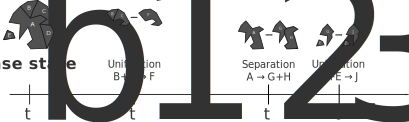
\includegraphics[width=0.8\textwidth]{graphics/basics/stdm/event-based_spatio-temporal_data_model}
%   \caption{The Event-Based Spatio-Temporal Data Model}
%   \label{fig:event-based_spatio-temporal_data_model}


A main problem is to maintain the integrity of the spatial topology when a new change gets inserted not at the end of the list. A simple example shows that problem: Given geo-object $X$ is part of the inital base configuration at change $t_b$. At a later change, e.g. $t_y$ $X$ gets replaced by object $Y$. If a new change that updates $X$ to $X'$ gets inserted before at time point $t_x < t_y$, then $t_y$ is not integer anymore, because object $X$ does not exist. That is why on insertion of a change, all succeeding changes have to be tested for integrity and it might be necessary to update later changes.

% subsection data_structure (end)

% section hivent_model (end)

% ==============================================================================
%!TEX root = ../masters_thesis.tex
\label{sec:development}

\section{Development} % (fold)

distributed Web-based system
classic approach: UI <-> Client (main program) <-> Server (middleware) <-> DB

% ------------------------------------------------------------------------------
\subsection{Data Input} % (fold)
\label{sub:input}

This HGIS needs data about historical countries, their names and borders and historical events that lead to historical changes of these countries. There are a lot of free and open sources for geographic data about the current countries, their names and borders. One of the most exhaustive collections of geographic data in public domain is hosted by Natural Earth
\footnote{
  \textit{Natural Earth},
  URL: \url{http://www.naturalearthdata.com/downloads/},
  last access: 30.10.2015
}.
There is physical data (e.g. coastlines, rivers, or glacier areas) and cultural data (e.g. political borders, cities, roads, airports or timezones). OpenStreetMap also opens its database to the public
\footnote{
  \textit{Planet OSM},
  URL: \url{http://planet.openstreetmap.org/},
  last access: 30.10.2015
}.

However, data about historical countries and events are not as straightforward to aquire, because of the mostly qualitative nature of historical research (see section \ref{sub:history}). The most exhaustive free and open source of historical is the \emph{Wikipedia} and their article categories, e.g. \texttt{armistices} or \texttt{treaties}
\footnote{
  \textit{Category:Treaties},
  Wikipedia, the free encyclopedia,\\
  URL: \url{https://en.wikipedia.org/wiki/Category:Treaties},
  last access: 13.05.2016
}.
All sorts of historical events can be found, even translated into different languages. Some information is structured in information boxes, e.g. some historical treaties have a name, an image, a location, a signature and an effect date, an overview about treaty conditions and signatories. Particularily interesting for this thesis are articles about historical countries
\footnote{
  \textit{List of former sovereign states},
  Wikipedia, the free encyclopedia,
  URL: \url{https://en.wikipedia.org/wiki/List_of_former_sovereign_states},
  last access: 13.05.2016
},
because they contain the name of the country and meta information, e.g. their historical successors and predecessors. Building an open-source Historical Geographic Information System on the basis of Wikipedia would be a huge project with significant impact on the world of free and open education --- however, it would also be a big challenge: Wikipedia is incomplete, not all historical countries and events necessary to model the history of the world are available. It is also inconsistent, because not all articles about historical countries and events are structured, especially not to those who actually have an influence on a territorial change of a country, e.g. a border agreement. Retrieving, parsing and processing this information is a big challenge. Also the problem of accuracy and quality of information in the Wikipedia due to their open source nature has to be considered. Overall, using the Wikipedia as a data source for this thesis is not feasible, but is subject to further research.

% - - - - - - - - - - - - - - - - - - - - - - - - - - - - - - - - - - - - - - -
\paragraph{Historical maps} % (fold)
\label{par:historical_map}

The most problematic data to acquire is about the territories and borders of historical countries. There is no primary data source for that, so the only way to retrieve a border is to extract it from an historical map.

They also can be found on Wikipedia, or in historical map colletions, e.g. \emph{OldMapsOnline}. The project is developed ``out of a love of history and heritage of old maps'' and currently stores about 400000 historical maps
\footnote{
  \textit{Old Maps Online},
  URL: \url{http://www.oldmapsonline.org/},
  last access: 13.05.2016
}.
There are five steps to retrieve a border with points in geographic coordinates from an historical map.
\begin{enumerate}
  \item \textbf{Digitization}: If the map is on paper, it has to be scanned in the best possible quality. The result is a raster graphic.
  \item \textbf{Georeferencing}: The historical map has to fit as good possible on the reference map. This requires to manually define a set of reference points which are used to transform the map into the geographic coordinate system. This process is error-prone, especially if the projection of the historical map is not known and the map itself is not accurate
  \cite[pp. xvii]{knowles2002past}.
  The outcome is a raster graphic in which each pixel is assigned a geographic coordinate.
  \item \textbf{Preprocessing}: The raster image has to be be processed so that the desired border stands out and can be traced in the next step. This happens via greyscale conversion, thresholding or the Canny Edge Detector. This results in a monochrome graphic in which the desired border must be uninterrupted and clearly be seen.
  \item \textbf{Line detection}: By selecting a start and an end point of the border, the line gets traced automatically. This step vectorizes one particular feature, a borderline, from the raster graphic and produces a polyline in geographic coordinates.
  \item \textbf{Postprocessing}: In the last step, the polyline can be adapted: The line can be simplified to reduce unnatural artifacts and the position of border points can be manually edited. The final output of the whole process is a polyline whose points are expressed in the geographic coordinate system which can be used in the system as a border of an historic country.
\end{enumerate}

This process was developed in a preceding \emph{HiBo} project
\footnotetext{
  \textit{HiBo - semi-automatic extraction of borders from historical maps},
  Project of: B. Weber, N. K. Dankwa, K. Singh and T. Kashyappan, supervised by: Prof. Volker Rodehorst and Marcus Kossatz, Bauhaus-Universität Weimar, February 2015,
  URL: \url{https://bitbucket.org/bastian_weber/hibo},
  last access: 29.10.2015
}
(see figure \ref{fig:hibo}).

\begin{figure}[ht]
  \centering
  \begin{subfigure}{0.48\textwidth}
    \centering
    \includegraphics[width=0.95\linewidth]{graphics/basics/hibo1.png}
    \caption{Georeferencing}
  \end{subfigure}
  \begin{subfigure}{0.48\textwidth}
    \centering
    \includegraphics[width=0.95\linewidth]{graphics/basics/hibo2.png}
    \caption{Semi-automatic digitizing}
  \end{subfigure}
  \caption{Semi-automatic extraction of a border from a map of the Roman Empire \protect\footnotemark}
  \label{fig:hibo}
\end{figure}

% paragraph historical_map (end)


% - - - - - - - - - - - - - - - - - - - - - - - - - - - - - - - - - - - - - - -
\paragraph{Manual data input} % (fold)
\label{par:manual_data_input}

For the domain of this HGIS, the development of countries over time, there is no complete dataset available. Therefore, the system developed in this thesis needs to have an interface to enter historical data. The user needs to have an interface to enter information about historical events that change territories and names of historical countries. This data has to be acuired either from primary historical sources directly, or from free online sources. Next to Wikipedia, there are other collections of historical events, e.g. \emph{Correlates of War}
\footnote{
  \textit{Data Sets},
  Correlates of War,
  URL: \url{http://www.correlatesofwar.org/data-sets/folder_listing},
  last access: 13.05.2016
}
for quantitative data about international relations.
% paragraph manual_data_input (end)

% subsection data_input (end)

% ------------------------------------------------------------------------------
\subsection{System Architecture} % (fold)
\label{sub:system_architecture}


The system developed in this thesis is Web-based. That means, there is a \emph{client}, a Web browser, and a remote Web \emph{server} with a database and a middleware. The Web browser hosts the applications user interface. If the user interacts with a tool the client sends a request to the Web server for new data. The middleware checks the request and queries the necessary data from the database. The data will be transformed and sendt back to the client. On the map and the timeline the new information will be shown.

This clear separation between the data (\emph{model}), the user interface (\emph{view}) and the middleware (\emph{controller}) follows directly from the \emph{model-view-controller pattern}: One part can be changed without interfering the other parts, e.g. if the 2D map is replaced by a 3D globe, only the view changes, but the middleware and the database can stay untouched. Likewise, the implementation of a new database technology has no consequences to the view.

graphic of basic system:
UI
Client-side mechanism
Server-side mechanism
Database

programming languages / Framworks
Client                    HTML
          Less ->         CSS
          CoffeeScript -> JavaScript
Server    Django ->       Python
                          PostgreSQL
                          + PostGIS

% subsection system_architecture (end)

% ------------------------------------------------------------------------------
\subsection{Edit Mode} % (fold)
\label{sub:edit_mode}


user operations     CRE     UNI          SEP         TCH         NCH      DES
                     |      / \         /   \        /  \       /   \      |
HG operations       CRE   UNI   INC   SEP   SEC   TCH   BCH   NCH   ICH   DES

area changes        ADD   DEL*  DEL*  DEL   TCH   TCH   TCH   NCH   ADD   DEL
ADD, TCH, NCH, DES        ADD   TCH   ADD*  NCH?        TCH         DEL
                                NCH?        ADD*


geometries must be edited



% subsection edit_mode (end)

% ------------------------------------------------------------------------------
\subsection{HistoGraph} % (fold)
\label{sub:histograph}

% subsection histograph (end)

% section histoglobe (end)


% ------------------------------------------------------------------------------
\subsection{Interface Design} % (fold)
\label{sub:interface_design}

human centered design

% - - - - - - - - - - - - - - - - - - - - - - - - - - - - - - - - - - - - - - -
\paragraph{Paper Prototype} % (fold)
\label{par:paper_prototype}

description of process
image of two prototypes

% paragraph paper_prototype (end)

% - - - - - - - - - - - - - - - - - - - - - - - - - - - - - - - - - - - - - - -
\paragraph{Mockup Prototype} % (fold)
\label{par:mockup_prototype}

description of process
screenshot of two steps in between and of final version

% paragraph mockup_prototype (end)

% - - - - - - - - - - - - - - - - - - - - - - - - - - - - - - - - - - - - - - -
\paragraph{Web Interface} % (fold)
\label{sub:final_version}

screenshot
explanation of all final UI Elements

% paragraph final_version (end)

% subsection interface_design (end)


% ------------------------------------------------------------------------------
\subsection{Client-Side Application} % (fold)
\label{sub:client_side_application}

Class diagram

HistoGlobe

SpatialDisplay -> Map

TimeController  <-> Timeline
                <-> NowMarker

HiventController                AreaController <->  AreasOnMap
HiventHandle                    AreaHandle
Hivent
HistoricalChange    AreaChange  Area
                                AreaName            AreaNameLayerOnMap
                                AreaTerritory       AreaTerritoryLayerOnMap

DatabaseInterface

EditMode -> EditOperation -> EditOperationStep
NewTerritoryTool* NewNameTool NewHiventBox
WorkflowWindow

HistoGraph

LabelManager*

important little utils
  Button, ButtonArea
  NumberInput, TextInput, TextInputArea
  Title
  Watermark
  DoublyLinkedList
  WithinTree
  Geometry -> Polypolygon -> Polygon -> Polyline -> Point


% subsection client_side_application (end)

% ==============================================================================
\subsection{Server-Side Application} % (fold)
\label{sub:server_side_application}

database model

           Hivent
             m
       HistoricalChange
             m
  --------AreaChange------
  |          |           |
  |     ----Area----     |
  m     m          m     m
AreaTerritory      AreaName

no transaction time, only valid / event time
only world time is regarded, not database time.

view

get\_all
save\_operation


% subsection server_side_application (end)

% section development (end)

% chapter concept (end)